% ----------------------------------------------------------
% MODELAGEM E DEFINIÇÕES TÉCNICAS
% ----------------------------------------------------------
\section{Modelagem e definições técnicas}
Está seção tem por objetivo demonstrar as modelagens e padronizações utilizadas no desenvolvimento da aplicação.

\subsection{Modelo Entidade Relacionamento}

\begin{figure}[H]
	\centering 
	\caption{\label{fig:mer}Modelagem Entidade Relacionamento}
	\includegraphics[width=\textwidth]{../imagens/Mer-estagiei.png} 
	\fonte{Os autores}
\end{figure}

\subsection{Diagrama Entidade-Relacionamento}

\begin{figure}[H]
	\centering 
	\caption{\label{fig:der}Diagrama Entidade Relacionamento}
	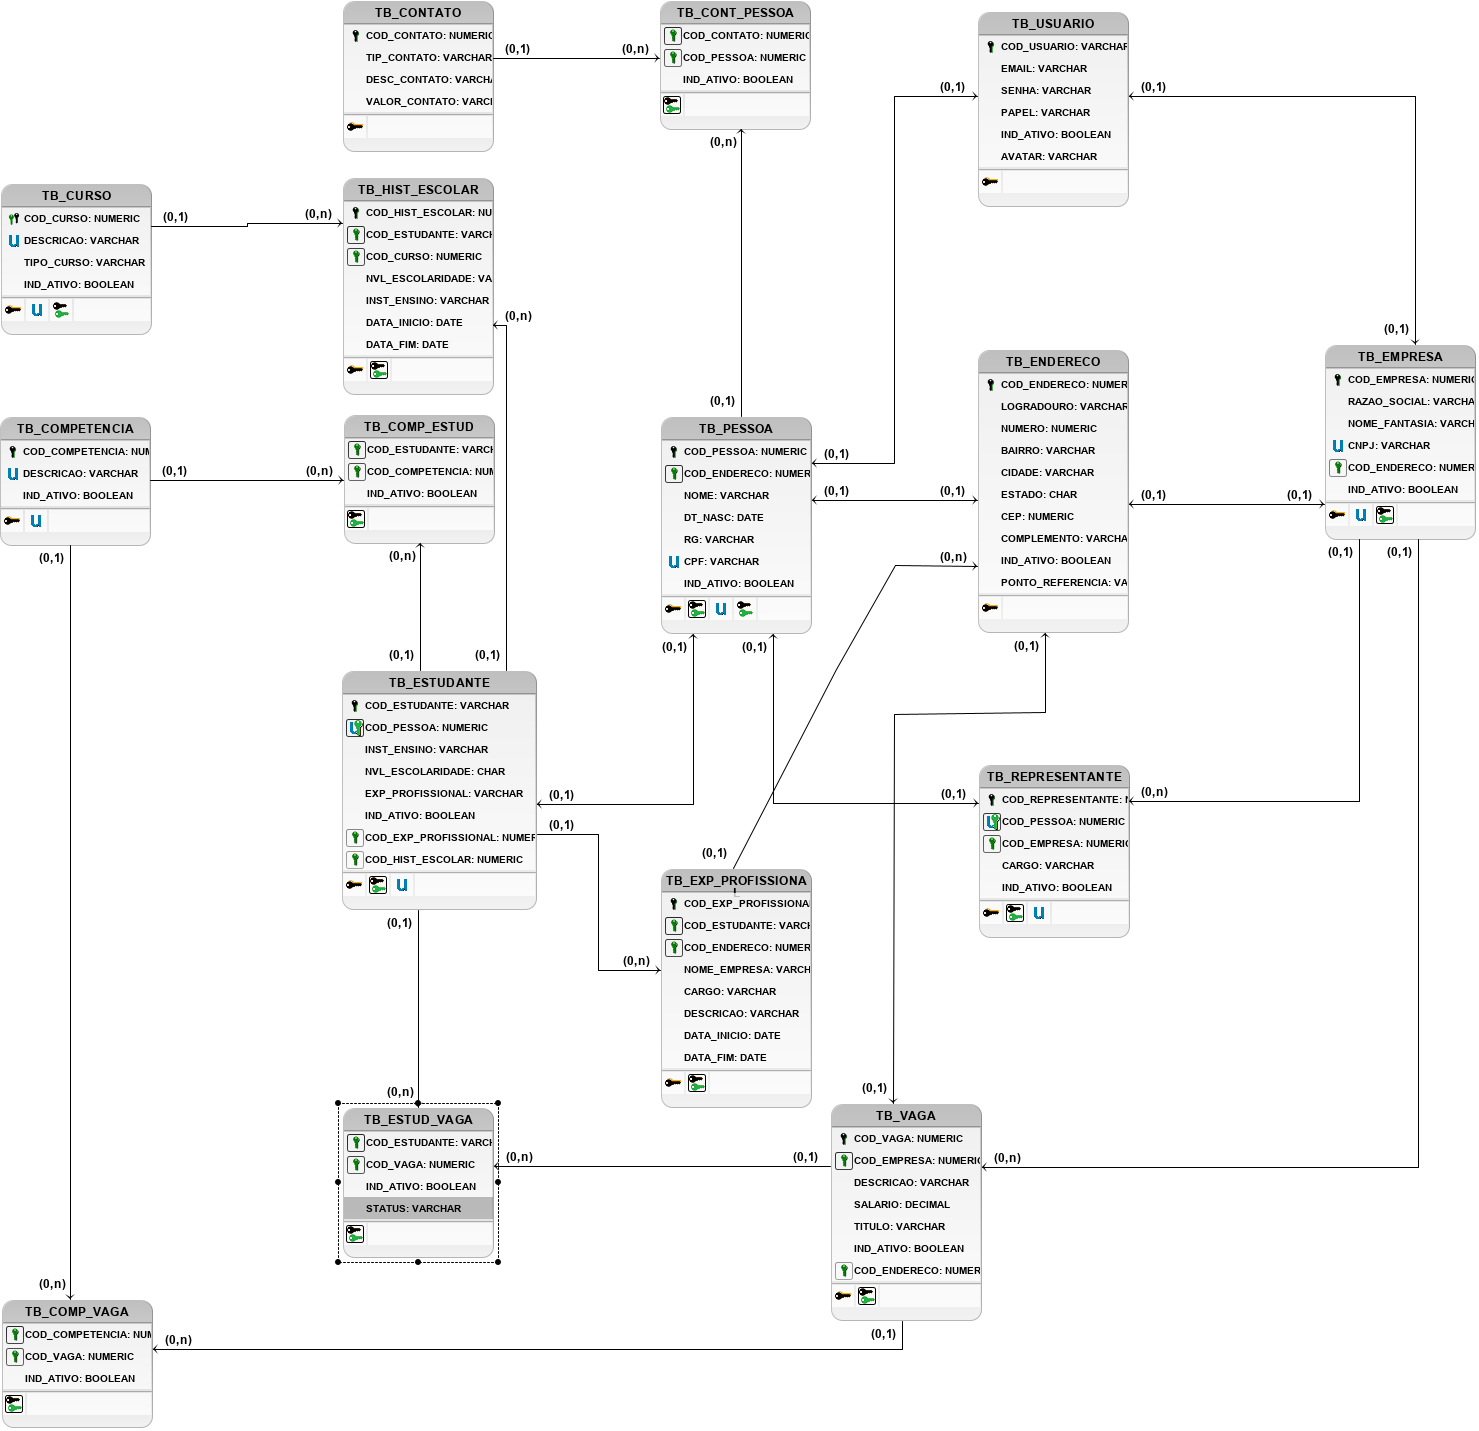
\includegraphics[width=\textwidth]{../imagens/der-estagiei.png} 
	\fonte{Os autores}
\end{figure}

\subsection{Dicionário de Dados}
A seguir mostramos as tabelas do nosso dicionário de dados.

\begin{figure}[H]
	\centering 
	\caption{\label{fig:dicio-leg}Legenda}
	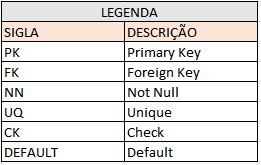
\includegraphics[width=0.6\textwidth]{../imagens/dicio-legenda.png} 
	\fonte{Os autores}
\end{figure}

\begin{figure}[H]
	\centering 
	\caption{\label{fig:dicio-user}Campos Usuário}
	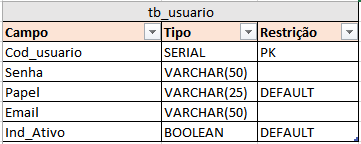
\includegraphics[width=0.8\textwidth]{../imagens/dicio-tb-usuario.png}
	\fonte{Os autores}
\end{figure}

\begin{figure}[H]
	\centering 
	\caption{\label{fig:dicio-person}Campos Pessoa}
	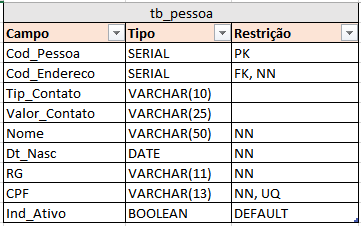
\includegraphics[width=0.8\textwidth]{../imagens/dicio-tb-pessoa.png} 
	\fonte{Os autores}
\end{figure}

\begin{figure}[H]
	\centering 
	\caption{\label{fig:dicio-student}Campos Estudante}
	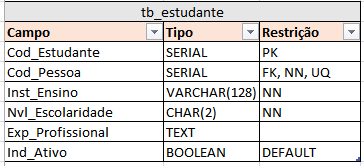
\includegraphics[width=0.8\textwidth]{../imagens/dicio-tb-estudante.png} 
	\fonte{Os autores}
\end{figure}

\begin{figure}[H]
	\centering 
	\caption{\label{fig:dicio-company}Campos Empresa}
	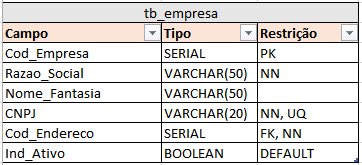
\includegraphics[width=0.8\textwidth]{../imagens/dicio-tb-empresa.png} 
	\fonte{Os autores}
\end{figure}

\begin{figure}[H]
	\centering 
	\caption{\label{fig:dicio-rh}Campos Representante RH}
	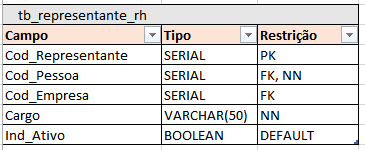
\includegraphics[width=0.8\textwidth]{../imagens/dicio-tb-representante-rh.png}
	\fonte{Os autores}
\end{figure}

\subsection{Endpoints da API}
%Endpoints -> \Glspl{endpoint}
%API -> \gls{api} ; APIs -> \glspl{api}
A seguir listamos os \glspl{endpoint} mapeados até o momento, com seus respectivos métodos de requisição \gls{http}.

\begin{quadro}[H]
	\caption{\Glspl{endpoint} da \gls{api}}
	\centering
	\begin{tabular}{| c | c | c |}
		\hline
		\thead{Classe Java}	& \thead{Método}	& \thead{Endpoint}		\\
		\hline
		LoginController			& POST				& /api/loginEstudante	\\
		\hline
		EstudanteController		& GET				& /api/estudante/\{id\}	\\
		\hline
		VagaController			& GET				& /api/vaga				\\
		\hline
	\end{tabular}
	\fonte{Os Autores}
	\label{endpoints}
\end{quadro}


\subsection{Listagem das Competências}
A seguir apresentamos as competências parametrizadas a fim de realizar a recomendação de vagas para os estudantes de acordo com seu perfil.

\begin{itemize}
	\label{softskills}
	\item Adaptação
	\item Atitude positiva
	\item Autoconfiança
	\item Autogestão
	\item Boa escrita
	\item Capacidade de resolver problemas
	\item Capacidade de tomar decisões
	\item Coaching
	\item Colaboração
	\item Comunicação
	\item Conhecimento político e cultural
	\item Criatividade
	\item Desenvolvimento da esquipe
	\item Desenvolvimento pessoal
	\item Empatia
	\item Estabelecimento de confiança
	\item Ética no trabalho
	\item Flexibilidade
	\item Gerenciamento de conflitos
	\item Honestidade
	\item Influência
	\item Inteligência emocional
	\item Interesse em aprender
	\item Liderança
	\item Motivação
	\item Organização
	\item Pensamento crítico
	\item Poder de negociação
	\item Proatividade
	\item Relacionamento interpessoal
	\item Resiliência
	\item Trabalho em Equipe
	\item Trabalho sob pressão
\end{itemize}